\documentclass[9pt, xcolor=table]{beamer}
%
% Packages
\usepackage[english]{babel} % Set language
\usepackage[T1]{fontenc}  % font Encoder for westeuropean languages
\usepackage[utf8]{inputenc} % Utf8 input encoder
\usepackage[autostyle=true,german=quotes]{csquotes} % quotation package
\usepackage[ddmmyyyy]{datetime} % for date and time formats
\usepackage[sorting=none,backend=biber]{biblatex}  % bibliography package
\usepackage{pgfpages} % print multiple pages per slide
\usepackage[font={footnotesize}]{caption} %caption package
\usepackage{xcolor} % color package
\usepackage{indentfirst}
%\usepackage{ziffer} % set , as decimal and . as thousand seperator (needed for german)
%
%
% activate to show notes on second screen:
%\setbeameroption{show notes on second screen}
%
%
% Bibliography
\addbibresource{references.bib} 
%
% Image Path
\graphicspath{{Images/}}    
%
% Style
% Define style
\usetheme{Boadilla}
\useoutertheme{miniframes}
\useinnertheme{rectangles}

% Define colours
\definecolor{THblack}{HTML}{000000}
\definecolor{THRed}{RGB}{201,12,15}
\definecolor{THOrange}{RGB}{234,91,12}
\definecolor{THPurple}{RGB}{184,37,133}
\definecolor{BlueSaphirre}{HTML}{0B4F6C}
\definecolor{DartmouthGreen}{HTML}{306B34}

% define element colors
\setbeamercolor{palette primary}{bg=THPurple,fg=white}
\setbeamercolor{palette secondary}{bg=THRed,fg=white}
\setbeamercolor{palette tertiary}{bg=THOrange,fg=white}
\setbeamercolor{palette quaternary}{bg=THblack,fg=white}
\setbeamercolor{structure}{fg=THblack}
\setbeamercolor{title}{fg=THRed}
\setbeamercolor{frametitle}{fg=THOrange}
\setbeamercolor{mini frame}{fg=white, bg=THOrange}
\setbeamercolor{section in head/foot}{fg=white, bg=THOrange}
\setbeamercolor{structure}{fg=THblack}

% define Block colors
\setbeamercolor{block title}{bg=BlueSaphirre!50, fg=white}
\setbeamercolor{block body}{bg=BlueSaphirre!15}
\setbeamercolor{block title alerted}{bg=THRed!50, fg=white}
\setbeamercolor{block body alerted}{bg=THRed!15}
\setbeamercolor{block title example}{bg=DartmouthGreen!55, fg=white}
\setbeamercolor{block body example}{bg=DartmouthGreen!15}

% define element styles
\setbeamertemplate{headline}{}
\setbeamertemplate{section in toc shaded}[default][50]
\setbeamertemplate{section in toc}[square]
\setbeamertemplate{subsection in toc}[square]
\setbeamertemplate{itemize items}[square]
\setbeamertemplate{enumerate items}[square]
\setbeamertemplate{caption}[numbered]
\setbeamertemplate{blocks}[default]

% Show numbers instead of symbols in bibliography
\setbeamertemplate{bibliography item}{\insertbiblabel}
\renewcommand*{\bibfont}{\small} % make font smaller

%The next block of commands puts the table of contents at the 
%beginning of each section and highlights the current section:
\AtBeginSection[]{
	\begin{frame}{Agenda}
		\tableofcontents[currentsection]
	\end{frame}
}

% restyle captions
\DeclareCaptionFont{grey}{\color{black!70}}
\captionsetup{
  labelfont={grey},
  textfont={grey}
}
%
% Title page information
\title[VIV introduction] {\LARGE{\textbf{Fluid Induced Vibration: VIV introduction.}}}

\author[Anonymous]{\Large{\textbf{Anonymous}}}
\institute[Master Student] {School of Mechanical Engineering and Automation
}
\newcommand{\Subject}{Group 3}
\newcommand{\PlaceAndTime}{Slides made in \insertdate}
%\newcommand{\Contactmail}{\url{21S153280@hit.stu.edu.cn}}
\newcommand{\Contactmail}{\url{\\}}
\newcommand{\StuId}{\\}
\date{\today}
%
% Title page of presentation
%
\makeatletter
\setbeamertemplate{title page}
{
	\vbox{}
	%
	\begin{center}
		\begin{minipage}[c]{0.8\linewidth}
			 
			\inserttitlegraphic
			    
			\begin{beamercolorbox}[sep=8pt,center]{title}
				\usebeamerfont{title}
				\inserttitle%
			\end{beamercolorbox}
			%
			\vspace{-2ex}\
			\begin{beamercolorbox}[sep=8pt,center]{author}
				\usebeamerfont{author}\small\insertauthor
				\vspace{3ex}
			\end{beamercolorbox}
			%
			\begin{minipage}[c]{.5\textwidth}
				\insertLogos
			\end{minipage}
			%
			\begin{minipage}[c]{.5\textwidth}
				\small
				
				\vspace{0.5em}
				
				\Subject\\
				
				\vspace{0.5em}
				
				\PlaceAndTime\\
				
				\vspace{0.5em}
				
				\insertinstitute
			\end{minipage}%
			%
		\end{minipage}
	\end{center}
}
\makeatother
% define title graphic
% \titlegraphic {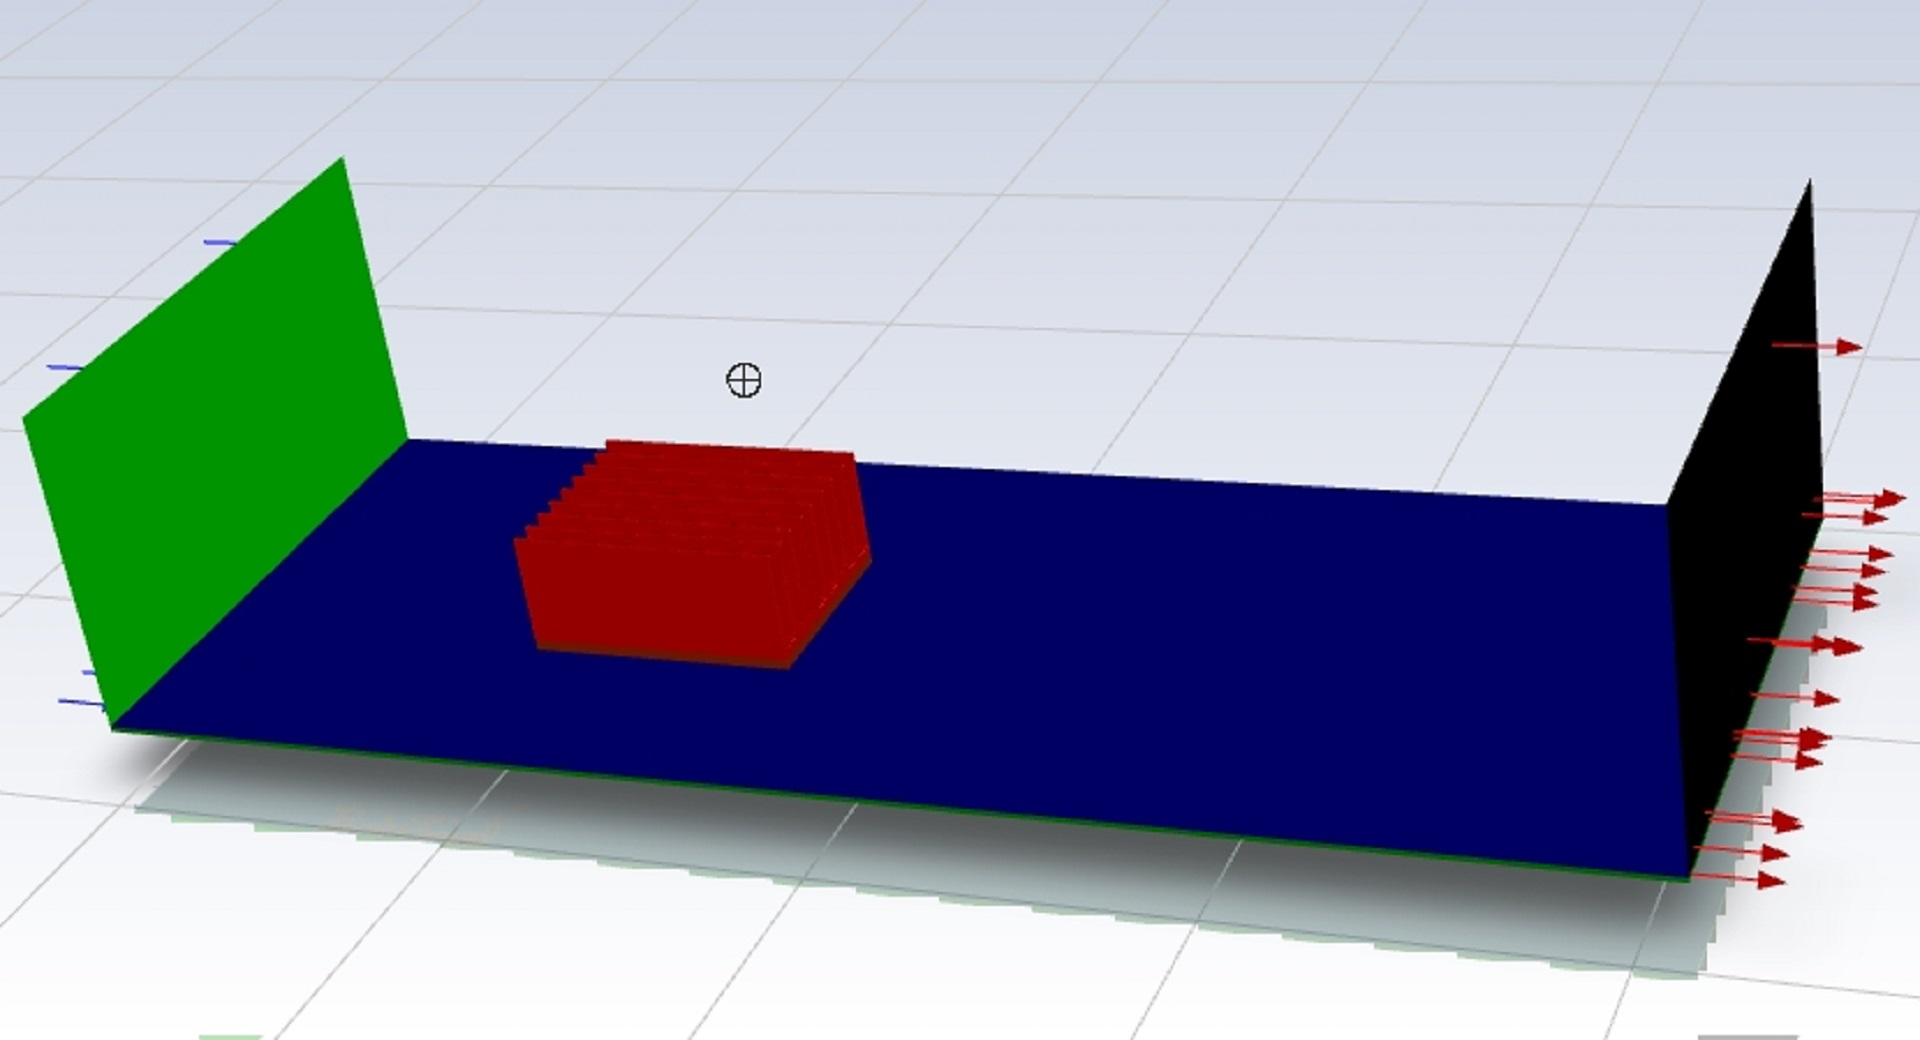
\includegraphics[width=\linewidth, trim={0 7cm 0 7cm}, clip]{title.jpg}}
\titlegraphic {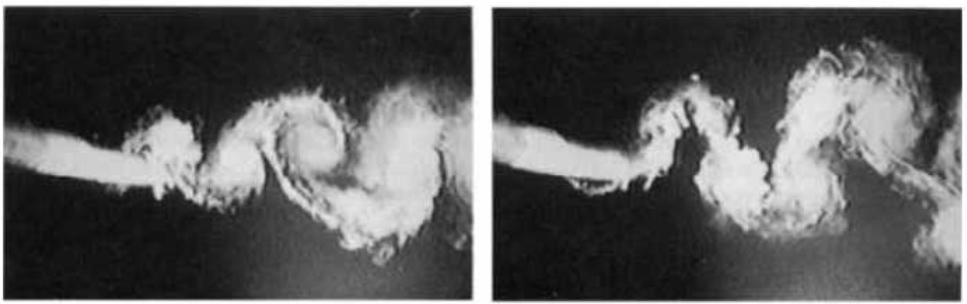
\includegraphics[width=\linewidth]{未标题-6.jpg}}
% title graphic logo
\newcommand{\insertLogos}
{\centering 
\includegraphics[height=1.5cm]{hitlogo.jpg}\hspace{1em}
\includegraphics[height=1cm]{wenzi-logo.png}}
%
% start of document
%------------------------------------------------------------------------------
\begin{document}
%
% Title page
\begin{frame}[plain]
	\titlepage
\end{frame}
%
\begin{frame}{Agenda}
	\tableofcontents
\end{frame}
%
%
\section{Introduction}
\begin{frame}{Fluid induced vibration}
	\begin{figure}
		\centering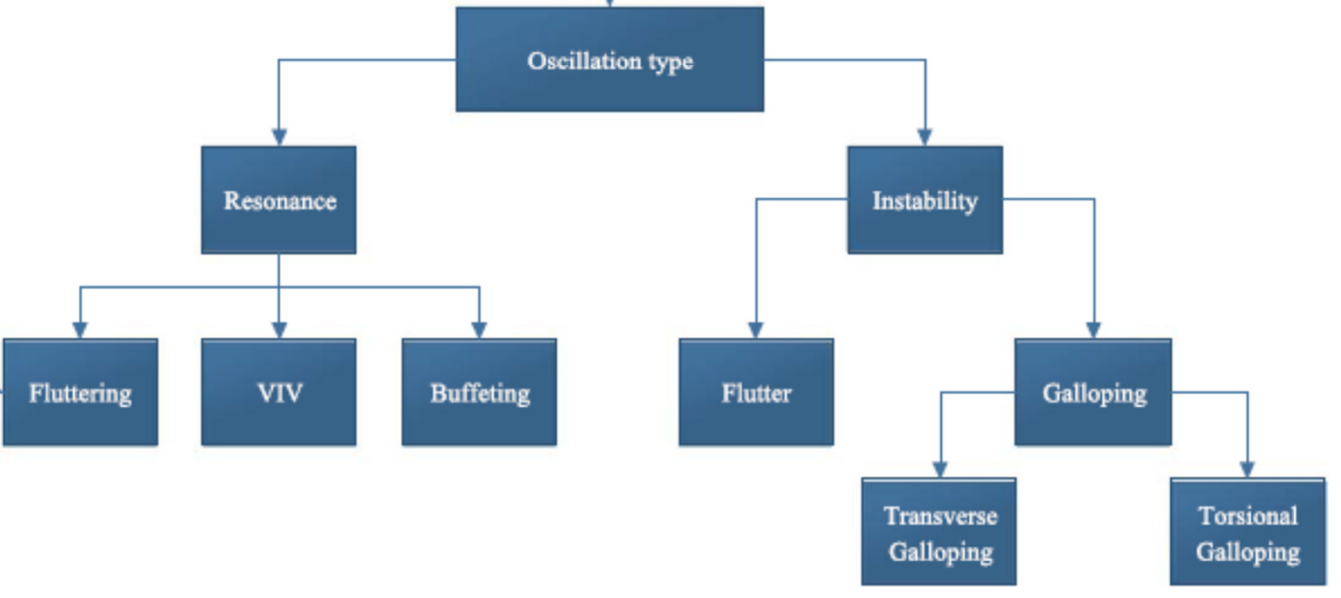
\includegraphics[height=5cm]{未标题-1.jpg}
		\caption{Classification of fluid-induced oscillation.}
	\end{figure}

	\centering
	\textbf{VIV: resonance induced by vortex shedding.}
\end{frame}
%
\section{VIV phenomenon}
\begin{frame}{Vortex induced forces}
	\begin{figure}
		\centering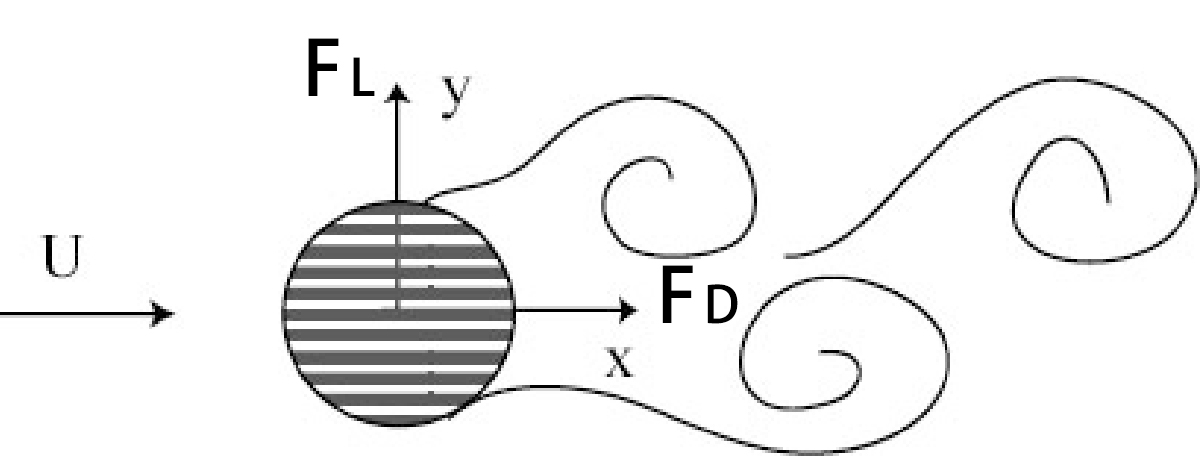
\includegraphics[height=3cm]{未标题-2.jpg}
		\caption{Vortex induced forces.}
	\end{figure}
	Force coefficients:
	\begin{equation}
		C_{D}=\frac{D(t)}{1 / 2 \rho U^{2} d} \quad C_{L}=\frac{L(t)}{1 / 2 \rho U^{2} d}
	\end{equation}

\end{frame}
\begin{frame}{Vortex induced forces}
	\begin{figure}
		\centering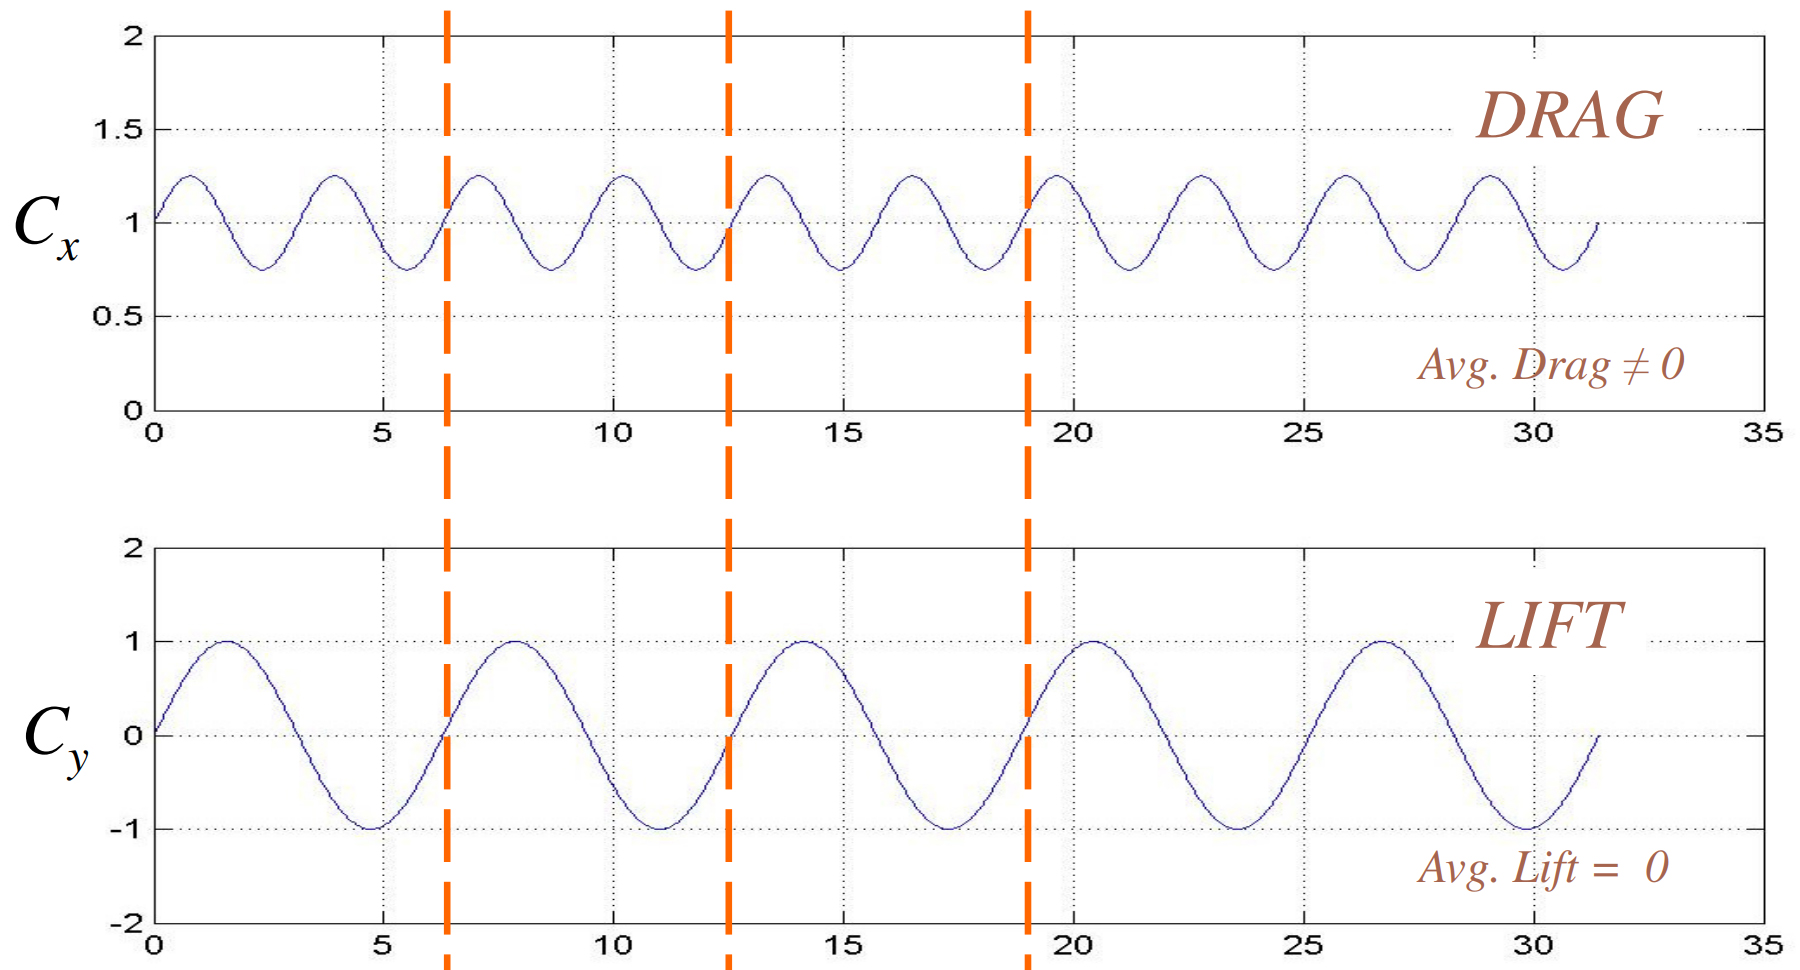
\includegraphics[height=4cm]{未标题-3.jpg}
		\caption{Force coefficients.}
	\end{figure}
	Frequency:
	\begin{equation}
		f_{C_{D}}= 2 f_{C_{L}}
	\end{equation}
\end{frame}
%
\begin{frame}{Parameters}
	\setlength{\parindent}{2em}
	\textbf{Input:}

	\vspace{1em}

	Mass ratio: $m^{*}=m / m_{f}$

	\vspace{1em}

	Damping ratio: $\zeta=c / c_{c}$
	\vspace{1em}

	Reduced velocity: $U r=U_{\infty} /\left(f_{n} D\right)$

	\vspace{1em}

	(Mass-damping ratio: $m^{*} \zeta=m^{*} c / c_{c}$)

	\vspace{2em}

	\textbf{Output:}

	\vspace{1em}

	Amplitude ratio: $A^{*}=A / D$

	\vspace{1em}

	Reduced frequency: $f^{*}=f_{v} / f_{n}$

	\vspace{1em}
\end{frame}
%
\begin{frame}{vortex excitation \& lock-in}
	\begin{figure}
		\centering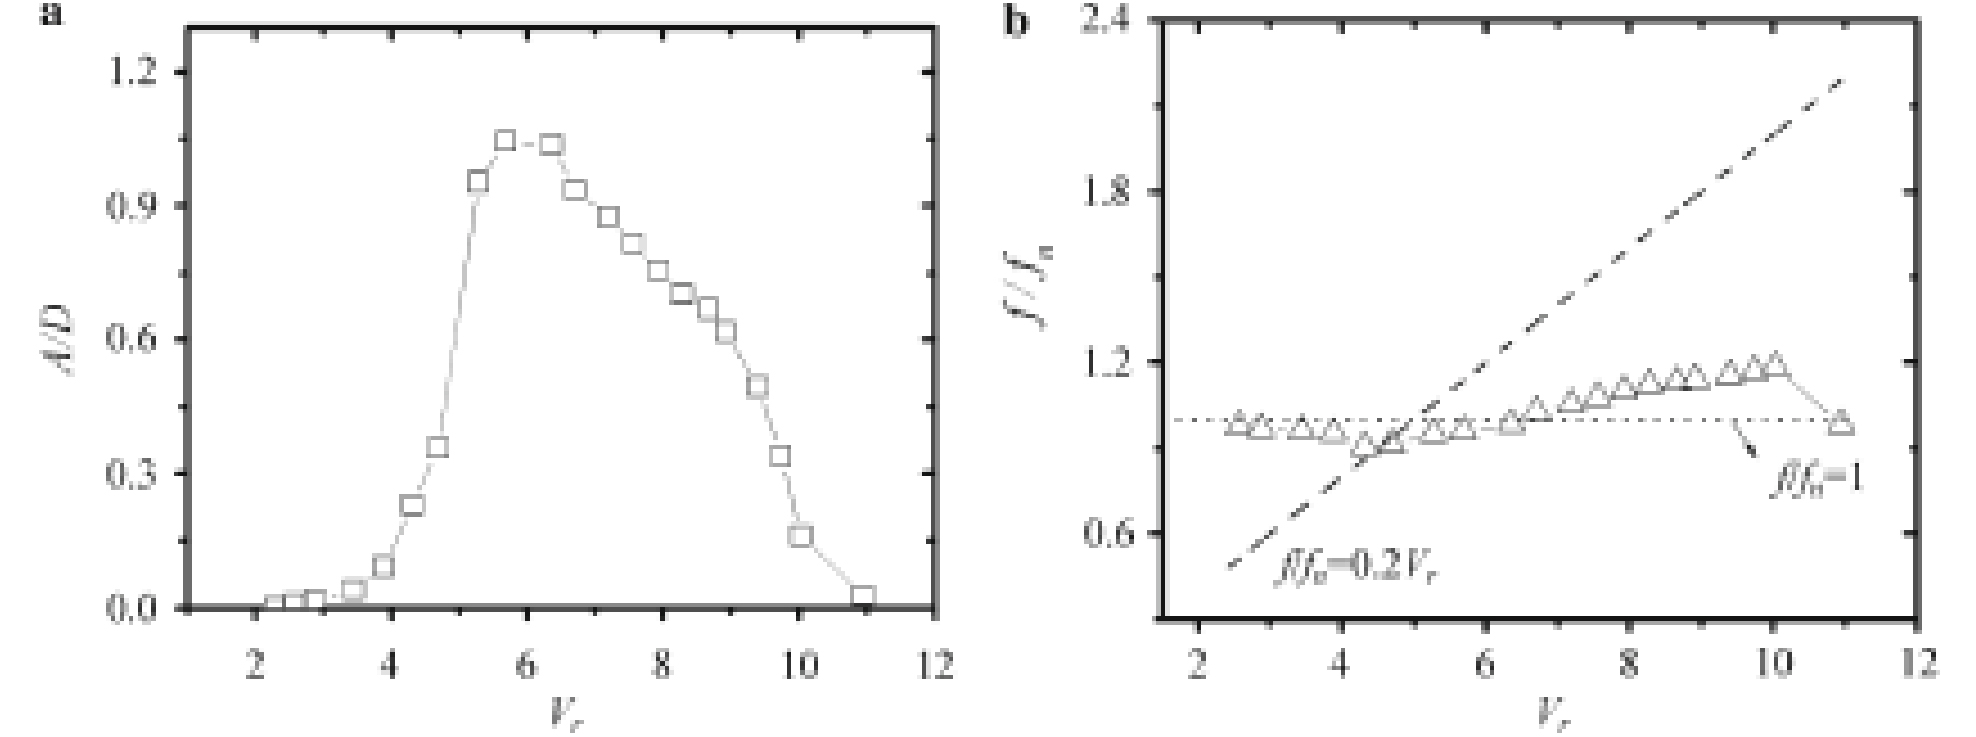
\includegraphics[height=4cm]{未标题-4.jpg}
		\caption{(a)$A^*-U_r$ (b)$f^*-U_r$}
	\end{figure}

	\setlength{\parindent}{2em}

	lock-in : when $f_v$ gets close to $f_n$, $f_v$ will remains at $f_n$ when $U_r$ is higher. (Resonance in Y dimension.)

	$A^*$ is effected by mass damping ratio $m^{*} \zeta$.
\end{frame}
%
\section{VIV linear analysis}
\begin{frame}{Linear analysis}	
	\setlength{\parindent}{2em}

	Forced damped system:
	\begin{equation}
		\begin{gathered}
		m \ddot{y}+c \dot{y}+k y=F_{L} \\
		y(t)=y_{0} \sin \omega t, \text { and }
		F_{L}(t)=F_{L 0} \sin (\omega t+\phi),
		\end{gathered}
	\end{equation}

	\vspace{0.5em}

	\begin{equation}
		F_{L 0} \sin (\omega t+\phi)=F_{L 0} \cos \phi \sin \omega t+F_{L 0} \sin \phi \cos \omega t
	\end{equation}

	\vspace{0.5em}

	Equation with the same form as a free damped vibration:

	\begin{equation}
		\left(m+\frac{F_{L 0} \cos \phi}{\omega^{2} y_{0}}\right) \ddot{y}+\left(c-\frac{F_{L 0} \sin \phi}{\omega y_{0}}\right) \dot{y}+k y=0
	\end{equation}

	Potential added mass \& damping:

	\begin{equation}
		m_{a}=\frac{F_{L 0} \cos \phi}{\omega^{2} y_{0}}, \text {   } c_{a}=-\frac{F_{L 0} \sin \phi}{\omega_{0}}
	\end{equation}



\end{frame}
%
\begin{frame}{Linear analysis}
	\setlength{\parindent}{2em}

	Reduced frequency:
	
	\begin{equation}
		f^*=\frac{\omega_o}{\omega_{n}}=\sqrt{\frac{m}{m_{t}}}=\begin{cases}
			< 1,& \phi < 90^{\circ} \\
			> 1,& \phi > 90^{\circ}
		\end{cases}
	\end{equation}

	In steady vibration case:

	\begin{equation}
		c_{total} = c-c_a =0
	\end{equation}


	Amplitude ratio (Flow around cylinder):

	\begin{equation}
		A^{*}=\frac{y_{0}}{D}=\frac{U_{r}^{2} C_{L 0} \sin \phi}{4 \pi^{3}\left(m^{*}+C_{A}\right) \zeta f^{*}}
	\end{equation}

	where $C_A = m_a/m_v$ is potential added mass coefficient, which is estimated as \textbf{1} for small amplitude and inviscid fluid.

	
\end{frame}
%
\begin{frame}{Added mass estimation}
	\setlength{\parindent}{2em}
	\begin{figure}
		\centering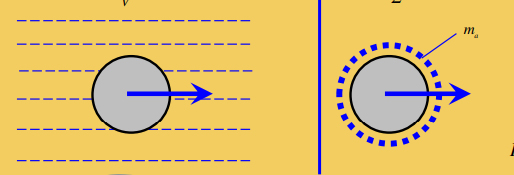
\includegraphics[height=2cm]{未标题-5.jpg}
		\caption{Cylinder in fluid(a) \& equivalent system (b)}
	\end{figure}	

	Kinetic energy: 
	\begin{equation}
		\begin{gathered}
		T=\frac{1}{2} \rho \int_{V}\left(u^{2}+v^{2}\right) d v
		=\frac{1}{2} m_{a} U^{2}
		\end{gathered}
	\end{equation}
	
	\noindent\begin{equation}
		\begin{aligned}
		m_{a} &=\rho \int_{V}\left(v_{r}^{2} / U^{2}+v_{\theta}^{2} / U^{2}\right) d v=\frac{\rho}{U^{2}} \int_{\theta=0}^{2 \pi} \int_{r=R}^{\infty}\left(\left(\frac{\partial \phi}{\partial r}\right)^{2}+\left(\frac{\partial \phi}{r \partial \theta}\right)^{2}\right) r d \theta d r \\
		&=\frac{\rho}{U^{2}} \int_{\theta=0}^{2 \pi} \int_{r=R}^{\infty}\left(\frac{U^{2} R^{4}}{r^{3}}\right) d \theta d r=\rho \pi R^{2} = m_v
		\end{aligned}
	\end{equation}
	\vspace{1em}

	\centering
	\Large\textbf{Potential added mass = Mass of displaced fluid}
	
\end{frame}

\begin{frame}{Energy Balance}
	\setlength{\parindent}{2em}

	Work done by lift force:
	\begin{equation}
		\begin{aligned}
		W_{f}&=\oint F_{L} d y \\
		&= \int ^T_0 {F_{L0}} \sin (\omega t + \phi) \cdot y_0 \omega \cos (\omega t) d t \\
		&=\pi F_{0} y_{0} \sin \phi
		\end{aligned}
	\end{equation}

	Work done by damping force:
	\begin{equation}
		\begin{aligned}
		W_{c}&= -\oint c \dot y d y \\
		&= \int ^T_0 c \omega ^2 y_0^2 \cos ^2 (\omega t) d t \\
		&=-\pi c \omega y_{0}^{2}
		\end{aligned}
	\end{equation}

	There is: 
	\begin{equation}
		W_f + W_c = 0
	\end{equation}

	\centering
	\textbf{
	Energy received from the fluid = Energy dissipated through the damper.}

\end{frame}
%


\begin{frame}{}
	\usebeamerfont{AAA}
	\begin{center}
		\Huge Thanks for your attention!\\[2ex] 
		% \small Please feel free to ask any questions
		% \vspace{10ex}
		
	\end{center}
\end{frame}
%
%------------------------------------------------------------------------------
\end{document}
